\section{Příklad 1}
% Jako parametr zadejte skupinu (A-H)
\prvniZadani{C}
\subsection{Výpočet $R_{ekv}$}

\begin{figure}[H]
    \centering
    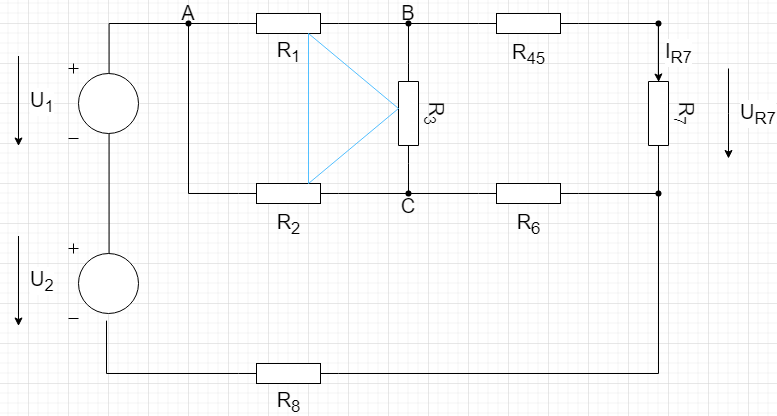
\includegraphics[scale=0.5]{picturesFor1Uloha/1.png}
    \caption{$R_4 + R_5$}
    \label{fig:Paralel_resistor_R45}
    \begin{quote}
    \centering
    $R_{45} =  \dfrac{R_4 * R_5}{R_4 + R_5} $  \\~\\~\\
    $R_{45} =  \dfrac{220\Omega * 220\Omega}{220\Omega + 220\Omega} = 
    \dfrac{48400\Omega}{440\Omega} = 110\Omega$
    \end{quote}
\end{figure}

\begin{figure}[H]
    \centering
    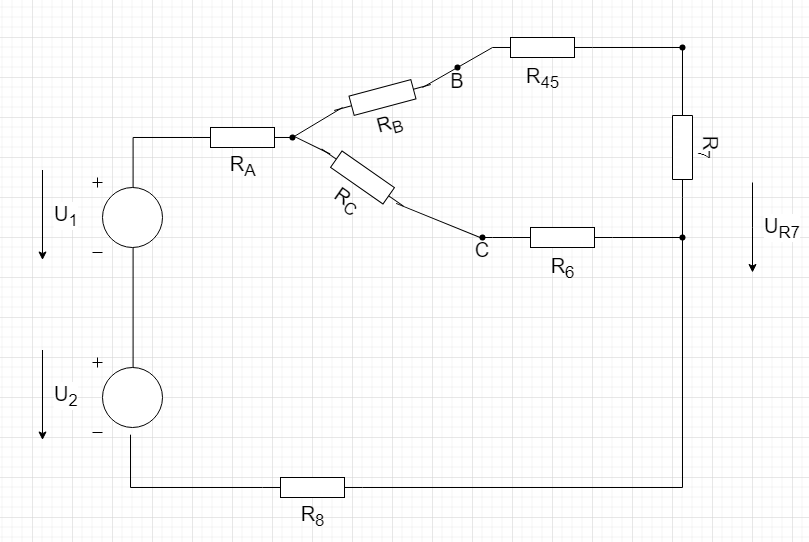
\includegraphics[scale=0.5, keepaspectratio]{picturesFor1Uloha/2.png}
    \caption{$Trojuhelnik \quad hvezda$}
    \label{fig:Trojuhelnik_Hvezda}
    \begin{quote}
    \centering
    $R_A =  \dfrac{R_1 * R_2}{R_1 + R_2 + R_3} $  \\~\\
    $R_B =  \dfrac{R_1 * R_3}{R_1 + R_2 + R_3} $  \\~\\
    $R_C =  \dfrac{R_3 * R_2}{R_1 + R_2 + R_3} $  \\~\\
    \medskip
    $R_A =  \dfrac{450\Omega * 810\Omega}{450\Omega + 810\Omega + 190\Omega} = \dfrac{364 500\Omega}{1450\Omega} = 251.3793\Omega$ \\~\\
    $R_B =  \dfrac{450\Omega * 190\Omega}{450\Omega + 810\Omega + 190\Omega} = \dfrac{85 500\Omega}{1450\Omega} = 58.9655\Omega$ \\~\\
    $R_C =  \dfrac{190\Omega * 810\Omega}{450\Omega + 810\Omega + 190\Omega} = \dfrac{153 900\Omega}{1450\Omega} = 106.1379\Omega$ \\~\\
    \end{quote}
\end{figure}

\begin{figure}[H]
    \centering
    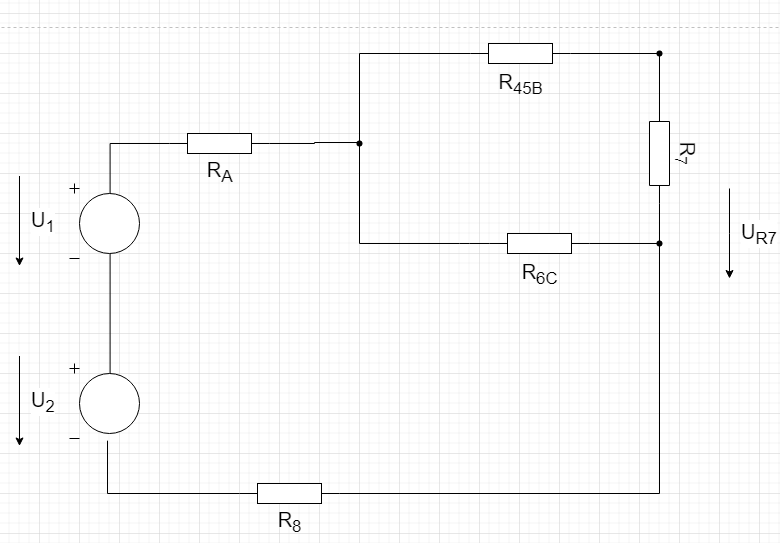
\includegraphics[scale=0.5]{picturesFor1Uloha/3.png}
    \caption{$Seriove \: zapojeni \quad R_{45} + R_B \quad a \quad R_6 + R_C $ }
    \label{fig:Serial_resistor_R45B_and_R6C}
    \begin{quote}
    \centering
    $R_{45B} = R_{45} + R_B $  \\~\\
    $R_{6C} = R_6 + R_C $  \\~\\
    $R_{45B} = 110\Omega + 58.9655\Omega = 168.9655\Omega$ \\~\\
    $R_{6C} =720\Omega + 106.1379\Omega = 826.1379\Omega$ \\~\\
    \end{quote}
\end{figure}

\begin{figure}[H]
    \centering
    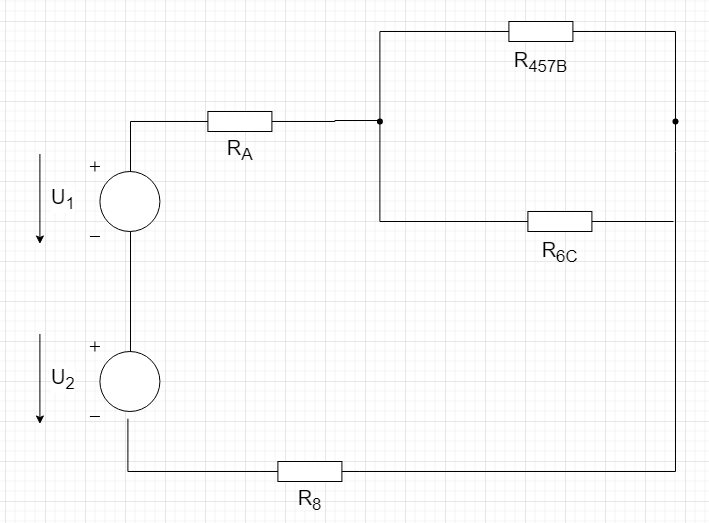
\includegraphics[scale=0.5]{picturesFor1Uloha/4.png}
    \caption{$ Zjednoduseni \: R_{45B} \: s \: R_7$}
    \label{fig:Serial_resistor_R457B}
    \begin{quote}
    \centering
    $R_{457B} = R_{45B} + R_7 $  \\~\\
    $R_{457B} = 168.9655\Omega + 260\Omega = 428.9655\Omega$
    \end{quote}
\end{figure}

\begin{figure}[H]
    \centering
    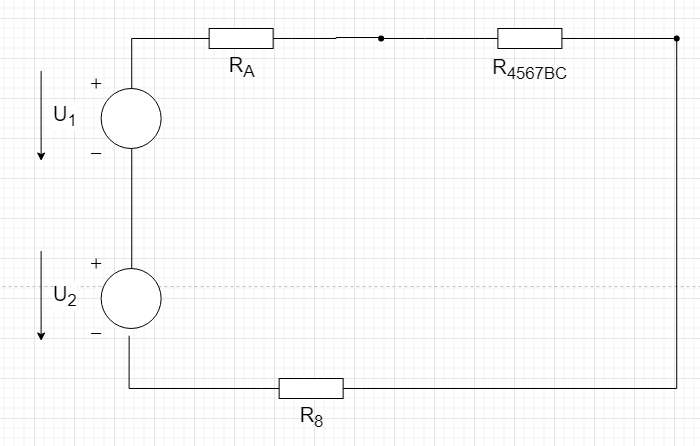
\includegraphics[scale=0.5]{picturesFor1Uloha/5.png}
    \caption{$Paralelne \: zapojene \: R_{457B} \: a \: R_{6C}$}
    \label{fig:Paralel_resistor_R4576BC}
    \begin{quote}
         \centering
        $R_{4576BC} =  \dfrac{R_{457B} * R_{6C}}{R_{457B} + R_{6C}} $  \\~\\~\\
        $R_{4576BC} =  \dfrac{428.9655\Omega * 826.1379\Omega}{428.9655\Omega + 826.1379\Omega} = \dfrac{354 384,6573\Omega}{1255.1034\Omega} = 282.3549\Omega $  \\~\\
    \end{quote}
\end{figure}

\begin{figure}[H]
    \centering
    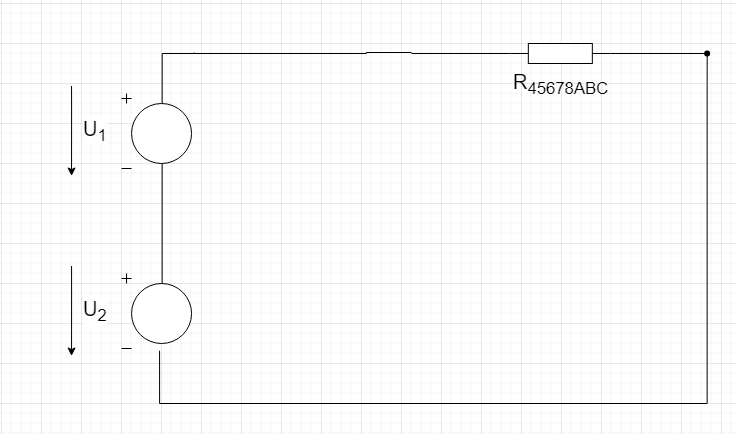
\includegraphics[scale=0.5]{picturesFor1Uloha/7.png}
    \caption{$ Zjednoduseni \: do \: R_{ekv}$}
    \label{fig:REKV}
    \begin{quote}
        \centering
        $R_{ekv} = R_{45678ABC} = R_A + R_{4567BC} + R_8$  \\~\\
        $R_{ekv} = R_{45678ABC} = 251.3793\Omega + 282.3549\Omega + 180\Omega = 713.7342 \Omega $  \\
    \end{quote}
\end{figure}
\begin{figure}[H]
    \centering
    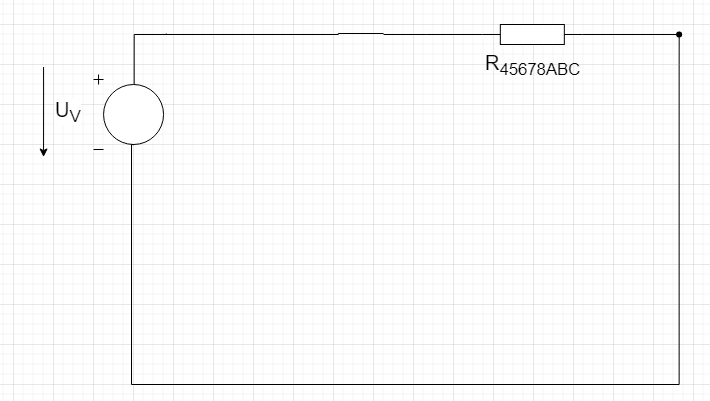
\includegraphics[scale=0.5]{picturesFor1Uloha/8.png}
    \caption{Vyhledávání U a I}
    \label{fig:Volt_and_Amper_founding}
    \begin{figure}[H]
	S $R_{ekv}$ nyní můžeme vypočítat celkový proud v obvodu Ohmovým zákonem: $I = \dfrac{U}{R_{ekv}}$
    \end{figure}
    \begin{quote}
        \centering
        $U_V = U_1 + U_2$ \\~\\
        $U_V = 100\Vo + 80\Vo = 180\Vo$ \\~\\
        $I = \dfrac{180\Vo}{713.7342\Omega} = 0.2521\Am$
    \end{quote}
\end{figure}


\subsection{Výpočet $U_{R7}$}

\begin{figure}[H]
    \centering
    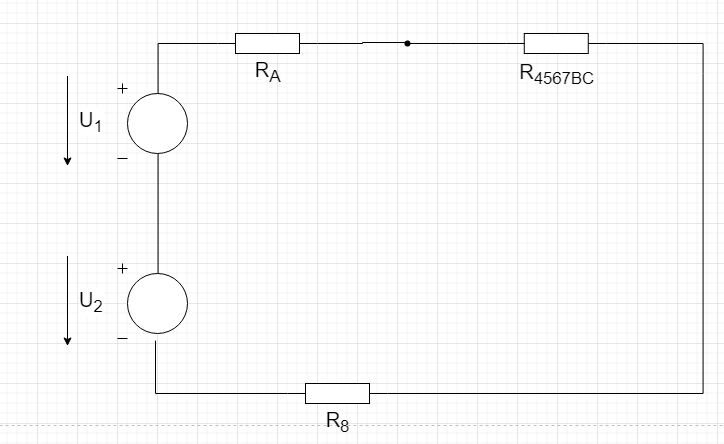
\includegraphics[scale=0.5]{picturesFor1Uloha/9.png}
    \begin{quote}
        \centering
	    Rozložíme zpětně obvod \\~\\
	    $U_{R4576BC} = I * R_{4576BC}$ \\~\\
	    $U_{R4576BC} = 0.2521\Am * 282.3549\Omega = 71.1816\Vo$ \\~\\
    \end{quote}
\end{figure}
\begin{figure}[H]
    \centering
    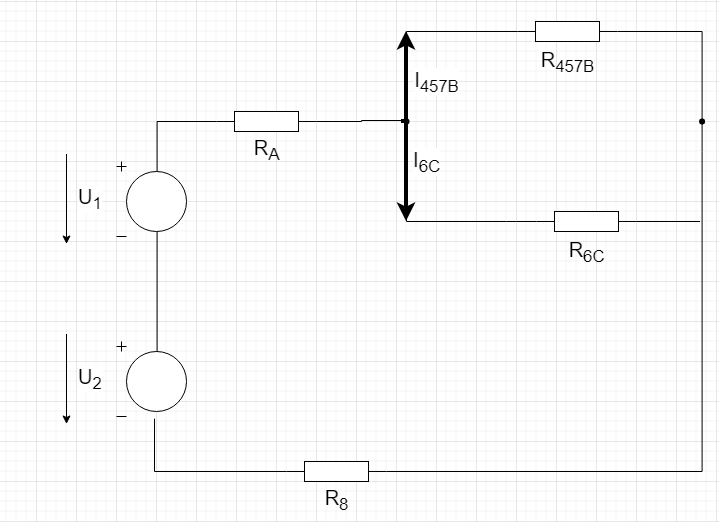
\includegraphics[scale=0.5]{picturesFor1Uloha/10.png}
    \begin{quote}
        \centering
        $I_{457B} = \dfrac{U_{R4576BC}}{R_{457B}} $ \\~\\
	    $I_{457B} = \dfrac{71.1816\Vo}{428.9655\Omega} = 0.1659\Am $ \\~\\
    \end{quote}
\end{figure}
\begin{figure}[H]
    \centering
    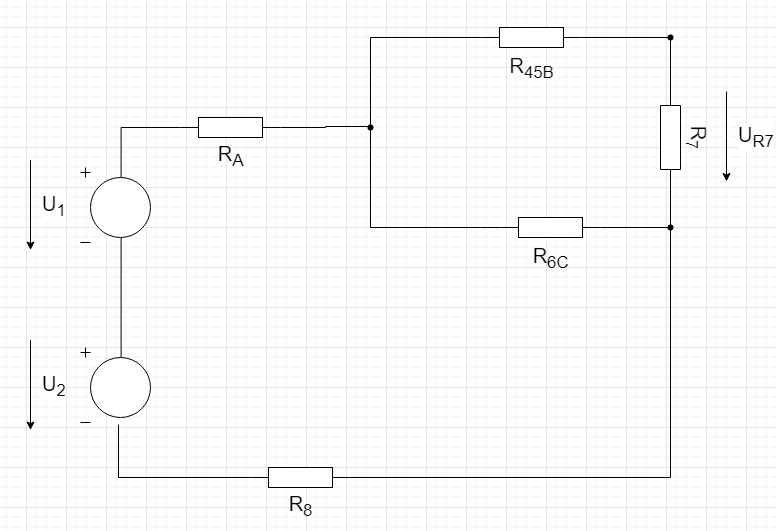
\includegraphics[scale=0.5]{picturesFor1Uloha/11.png}
    \begin{quote}
        \centering
         $I_{457B} = I_{R7} = 0.1659\Am $ \\~\\
         $U_{R7} = I_{R7} * R_{7}$ \\~\\
         $U_{R7} = 0.1659\Am * 260\Omega = 43.1438\Vo$ \\~\\
    \end{quote}
\end{figure}